\chapter{Detection of dynamic gestures}

\section{Proposed methods}

The dynamic gesture recognition problem is a problem, where the input data consist of several consecutive positions and orientations of hand and fingers. 
Moreover, the important factor for recognition is the time dependencies between sequences of hand positions.
The another challenge comes with the fact, that the gestures performed slower and faster should be recognized as the same dynamic gesture.

The proposed solution utilizes parts of the solution used for recognition of the static gestures.
Each frame of the captured data is described by the same features as in the static recognition part.
The set of features for each frame is then processed by the Hidden Markov Model scheme. 

\subsection{Hidden Markov Model}

Hidden Markov Model is model of a system (usually presented as a graph) with Markov property.
The Markov property means that the future state depends only on the following state and performed action.
The first introduction of HMM comes from the L. E. Baum et al.\cite{hmmfirst}, who proposed the mathematical background for HMMs.
A HMM can be considered a finite, $N$-element set of states (graph), which are associated with the probability distribution.
The transitions between states are represented by the transition probabilities usually stored in $N \times N$ matrix $T$.
In every state, one of the observation from the finite, $K$-element observation set can be generated with observation probability usually represented by the $N \times K$ emission matrix $E$.
The finite set of all possible observation is called the alphabet.
The HMM also consist of a $N$-element vector of initial state probabilities $\Pi$ of the hidden starting state.
Each HMM can be fully defined by the ($T$, $E$, $Pi$).

\begin{figure}[htb]
\centering
 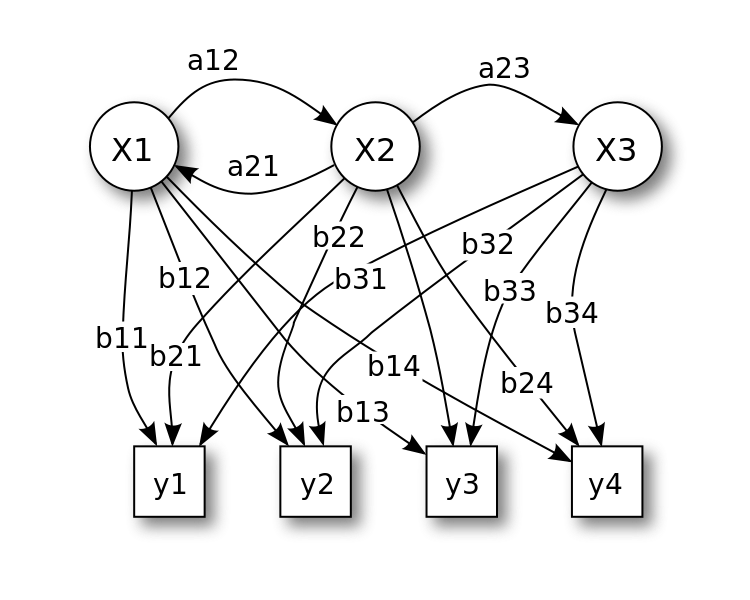
\includegraphics[width=0.8\columnwidth]{figures/HMM_wiki.png}
 \caption[]{Solution blocks of learning and testing parts in task of dynamic gesture recognition\footnotemark}
 \label{dynamicgestureswiki}
\end{figure}

\footnotetext{\url{http://en.wikipedia.org/wiki/File:HiddenMarkovModel.svg}}

The example HMM can be seen at fig.~\ref{dynamicgesturewiki}.
The HMM at the figure consists of 3 states ${X1, X2, X3}$ and 4 possible observations ${y1, y2, y3, y3}$.
The probabilities $a_{ij}$ define the transition probability from state $j$-th to state $i$-th. 
The probabilities $b_{ij}$ define the observation probability of generating $j$ observation while being in state $i$.

The HMM can be understood as a directed graph with two types of weighted vertices. 
This way, each state is represented by one type of vertices while observations can be shown as second type of vertices.
The edges between states contain and are an equivalent to the transition matrix. 
There are no edges between vertices representing observations.
The probability values for edges between states and observations are stored in the observation matrix.

There are three main algorithms used with the HMMs:
\begin{itemize}
\item Forward-Backward algorithm, 
\item Viterbi algorithm,
\item Baum-Welch algorithm.
\end{itemize}

The Forward-Backward algorithm is used to find the posterior probability of given states given the set of observations.
For the whole set of state variables $X = {X_i}_{i=1}^{N}$ and a sequence of observations $o_{1:t} = o_1, o_2,...,o_t$, the algorithm computes the $P(X_i | o_{1:t})$.
The algorithm utilizes a dynamic programming approach, by performing 3 steps in a loop: 
\begin{enumerate}
\item computing forward probabilities,
\item computing backward probabilities,
\item computing smoothed values.
\end{enumerate}
Firstly, the forward pass phase for $i=1,..,N$ computes the $P(X_i, o_{1:k})$, where $k$ is smaller than $t$, which represent the probability of ending up in state $X_i$ after first $k$ observations. 
The backward pass computes the $(P(o_{k+1:t}) | X_i)$, which are the probabilities of observing the rest of the observations in state $X_i$.
The smoothing part uses Bayes rule to compute the probability of state $X_i$ given the whole observation sequence:
\begin{equation}
P(X_k | o_{1:t}) = P(X_k | o_{1:k}, o_{k+1:t}) \propto P(o_{k+1:t} | X_k) P(X_k | o_{1:k})
\end{equation}
The time complexity of this algorithm is $O(N^2 T)$, where $T$ is the length of observation sequence and $N$ is the number of possible states.

The Viterbi algorithm is used to find the most likely sequence of hidden states that best explain (with maximum likelihood) the set of observations.
The set of those states is usually called the Viterbi path. 
Introducing the sequence:
\begin{equation}
V_{1,k} = P(o_1 | k) * \Pi_k)
\end{equation}
\begin{equation}
V_{t,k} = P(o_t | k) * argmax_{x\in X}(a_{x,k} * V_{t-1,x})
\end{equation}
The problem can be also understood as finding the $argmax_{x\in X}(V_{T,x})$. 
The algorithm time complexity is the same as forward-backward $O(N^2 T)$.

The Baum-Welch algorithm is the algorithm used to find the unknown parameters of the HMM.
For each training example, the algorithms computes the state transition probabilities, observation probabilities in each state and initial probabilities, which maximize the likelihood of observation.
Having the set of sets of observations, the algorithm can be used to train HMM to detect the sequences similar to the ones used in learning process.

\begin{figure}[htb]
\centering
 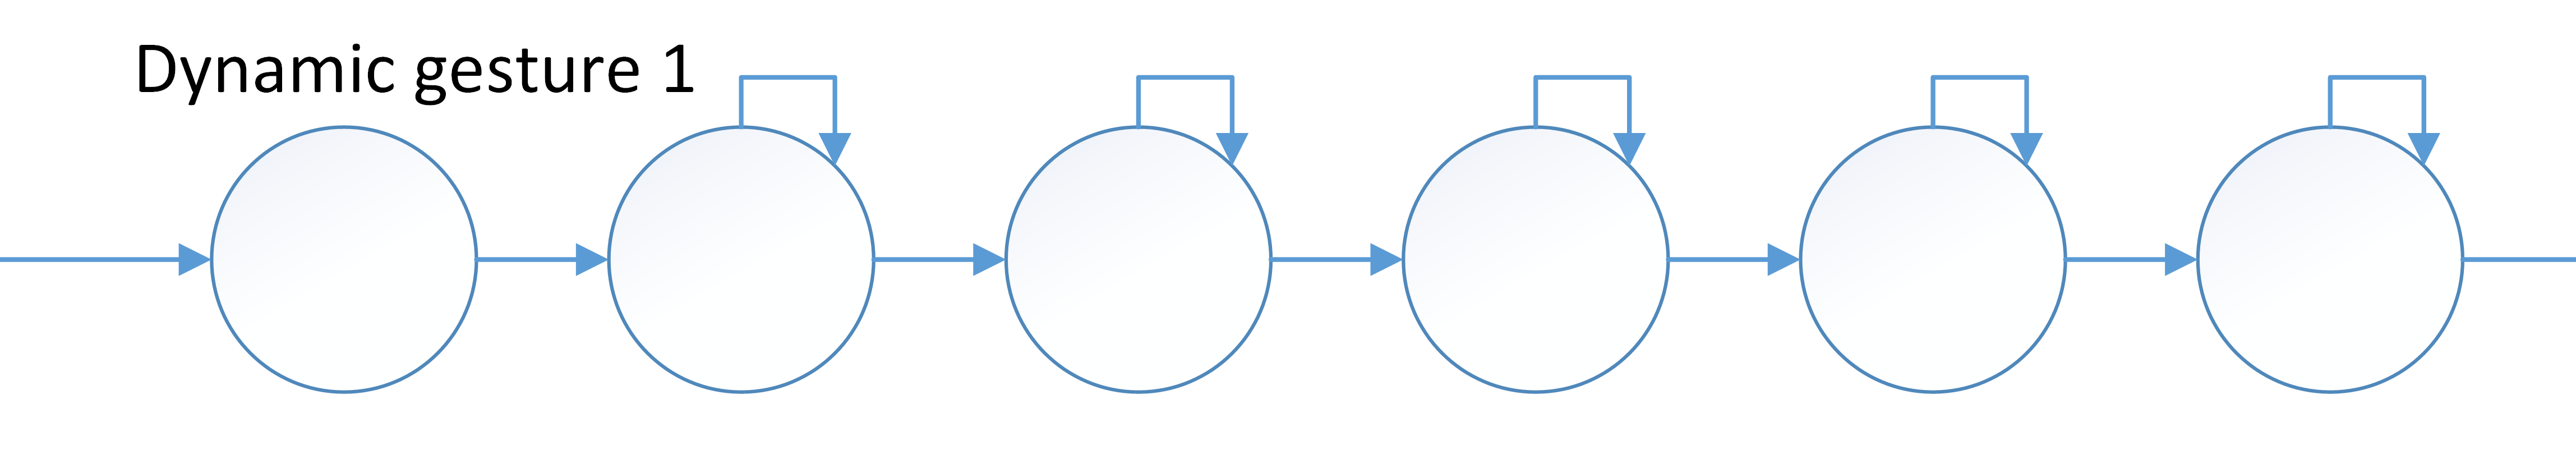
\includegraphics[width=1\columnwidth]{figures/SingleHMM.png}
 \caption{Non-zero state transitions and states of the HMM used to detect single dynamic gesture}
 \label{singlehmm}
\end{figure}

In the dynamic gesture recognition task, we adopted a structure of HMM with state having non-zero transition probabilities to itself and to the next state in the sequence.
The proposed structure is presented at fig.~\ref{singlehmm} and was firstly proposed in paper~\cite{hmm}.
The states can be understood as the phases of hand movement that happen when the wanted gesture is performed.
The self-transitions are used to model the different speeds of the gestures and thus allow to achieve more robust system.
This structure after training process can be used to measure the probability that the dynamic gesture occurred given the set of observations.

\begin{figure}[htb]
\centering
 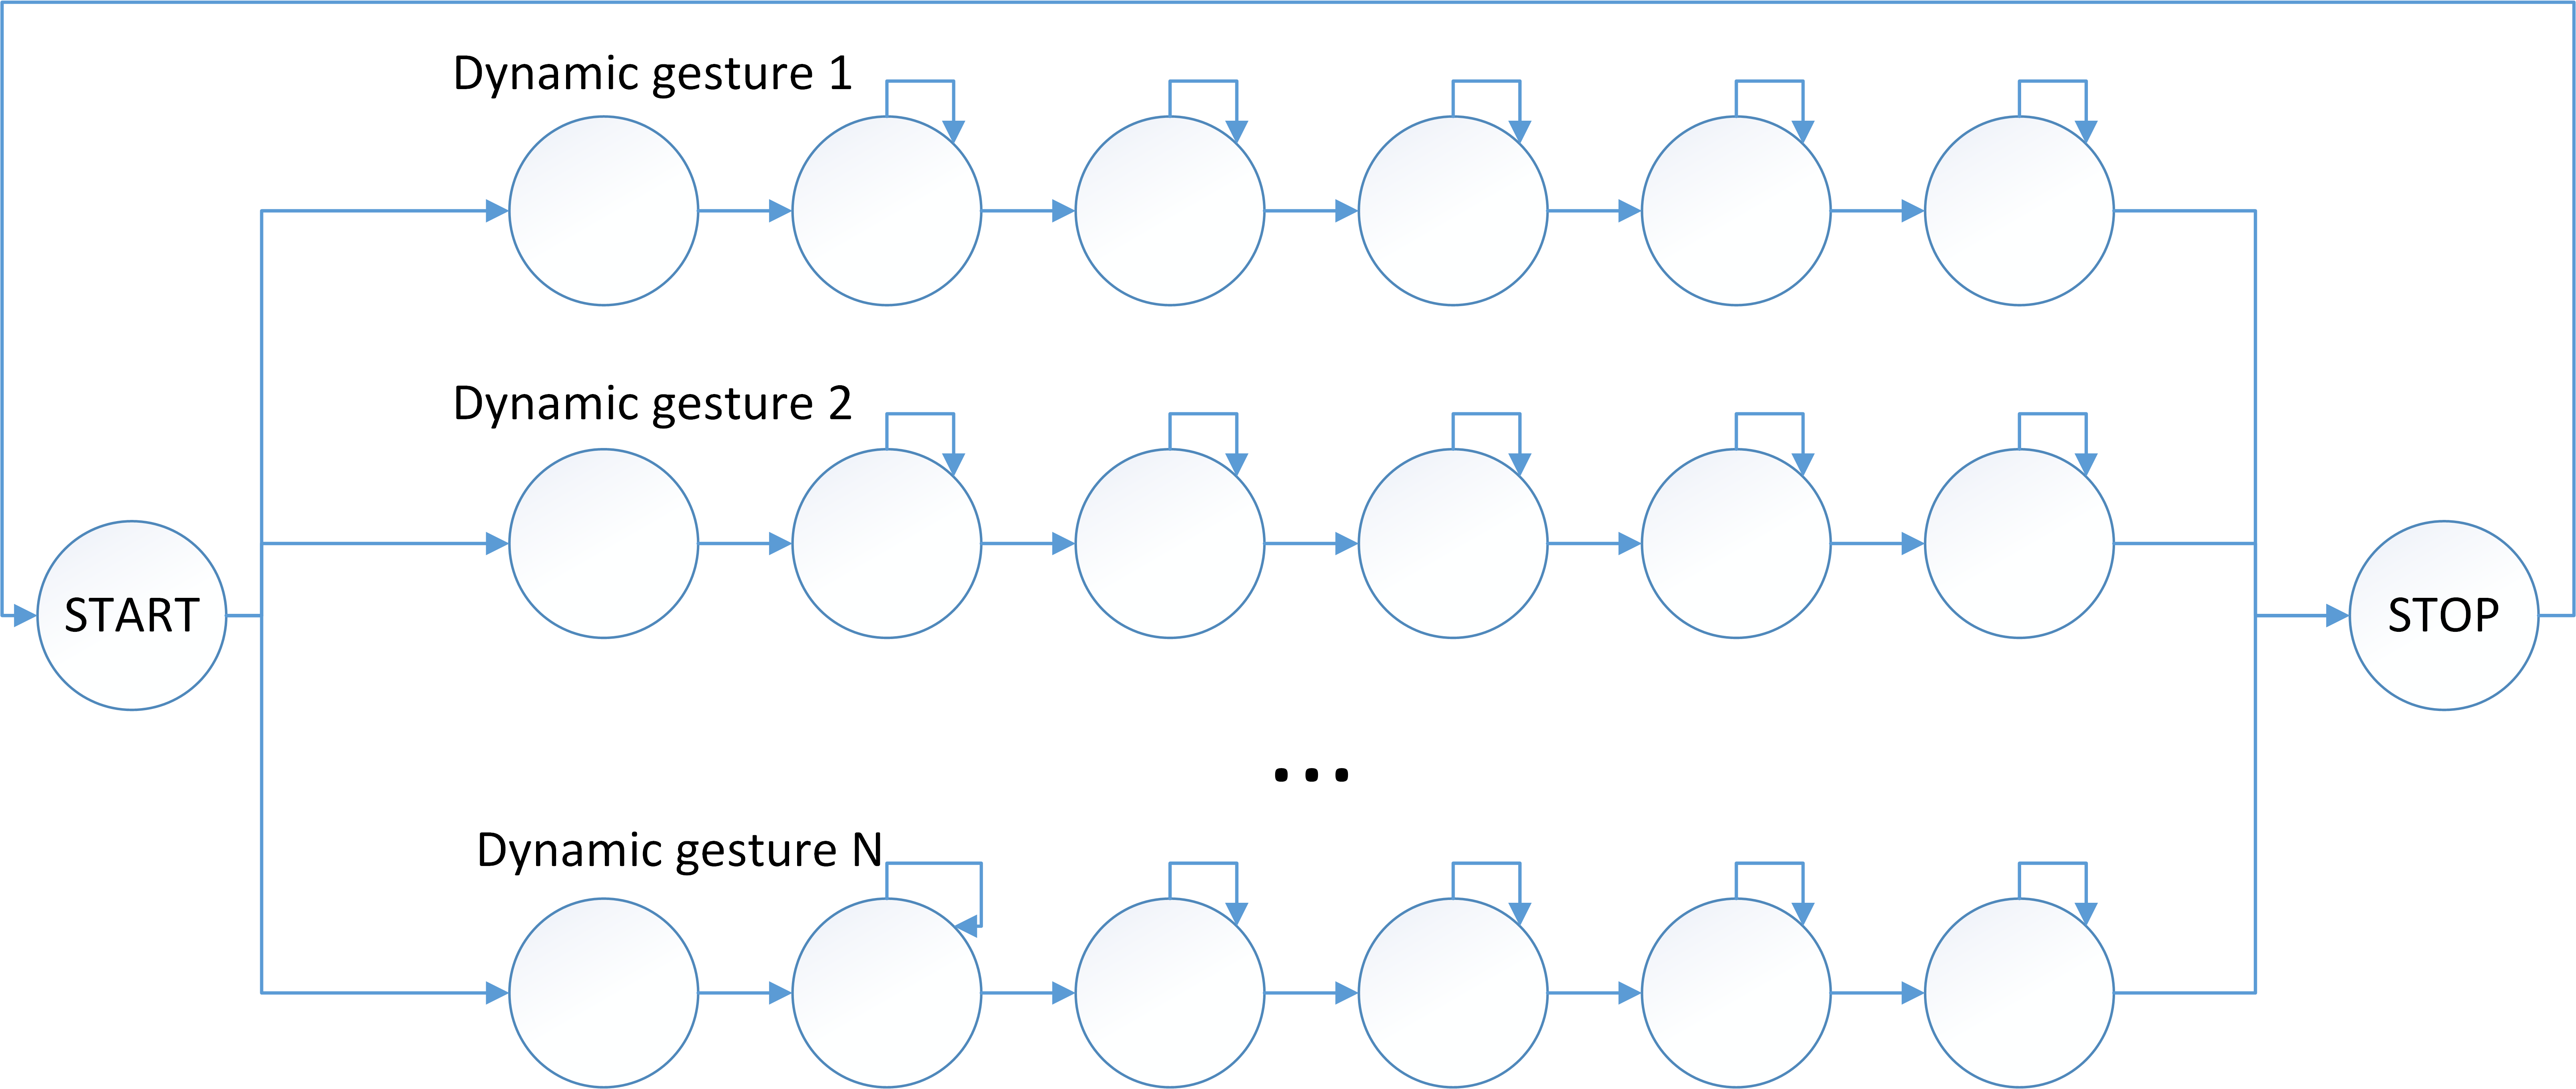
\includegraphics[width=1\columnwidth]{figures/HMM_eng.png}
 \caption{Non-zero state transitions and states for the HMM enabling simultaneous detection of $m$ dynamic gestures}
 \label{HMMstructure}
\end{figure}

Having single dynamic gesture recognition problem modelled as the sequence of $n$ states in which $k$-th state is connected by the edges to the $k$ and $(k+1)$ state and to the all observations.
Having the problem of distinguishing $m$ gestures translates to the problem of computing probabilities for $m$ sequential graphs.
The problem of finding if and what dynamic gesture occurred is the problem of finding the probabilities from each $m$ HMM.
Alternatively, the $m$ HMMs can be combined into one HMM were those single HMMs are treated as parallel paths.
The structure of proposed single HMM is presented at fig.~\ref{HMMstructure}.
Then the recognition process is a process of finding, which of the parallel paths is the most probable.

\subsection{HMM observation from Leap Motion data}

One of the problems when designing the system is a problem of correctly preparing the set of observations from the Leap Motion data.
Most of the proposed solutions in the literature assume that the observations are 1-dimensional.
This poses a challenge as the raw data from Leap Motion is high-dimensional.
That is the reason, why it is needed to reduce the dimensionality of the observation of the single hand in the predefined moment in time.

To do this, unsupervised clustering algorithms were introduced. 
For this task we examined 3 methods:
\begin{itemize}
\item Chinese whispers \cite{CW1, CW2},
\item Girvan-Newman clustering \cite{Newman},
\item k-means with additional methods to determine the number of clusters. \cite{kmeans1, kmeans2}.
\end{itemize}

Chinese whispers algorithm is an efficient randomized graph-clustering algorithm, which is time-linear in the number of edges.
The algorithm was proposed in \cite{CW1} and thoroughly examined in Natural Language Processing problems. 
The main advantage of the algorithm is the ability to independently determine the number of classes. 
In tests, we used the implementation available in dLib-ml library\cite{dlib}, which provides multiple machine learning algorithms.

Girvan-Newman clustering is a hierarchical algorithm used to detect clusters in a data represented as a graph.
The algorithm progressively removes edges from the original network until it reaches the maximal number of iterations or the error condition is met.
The solution iteratively calculates the eigenvalues of a created matrix using the power iteration method. 
In case of a complete graph, this algorithm is relatively slow.

The another proposed approach is a k-means clustering algorithm.
The idea for the algorithm comes from polish mathematician Hugo Steinhaus, but the first practical application has been presented in \cite{kmeans2}.
The algorithms initially randomly selects $k$ starting points and performs iteratively 2 steps utilizing the idea of expected-maximization \cite{expectedmaximization}:
\begin{enumerate}
\item For each data sample the algorithm calculates the distances to $k$ centroids and labels the samples with the label of the centroid with the smallest distance.
\item For each class, the algorithm recalculates centroids position to the averaged position of all samples belonging to class.
\end{enumerate} 
The algorithm stops after maximum number of iterations or when the change between consecutive iterations is smaller then defined epsilon.
Unfortunately, the algorithm requires the knowledge of the number of expected classes.
Although there exists a heuristics methods aiding in correctly choosing the number of classes. 
One of those methods is plotting the error sum of squares (SSE) within classes against the number of chosen classes. 
In this plot the drastic drop of SSE is sough and the number of classes it happens is considered a good choice.
Another, more formal approach introduces the measure of dissimilarity and is called Silhouette width \cite{silhouette}.
Declaring $a(i)$ as the average dissimilarity with all the other data within the same cluster and $b(i)$ as the lowest average dissimilarity to any other cluster which $i$ is not a part of, we can write a measure:
\begin{equation}
s(i) = \frac{b(i) - a(i)}{\max{\{a(i),b(i)}\}}
\end{equation}
The big value of $s(i)$ implies good clustering, while small value of $s(i)$ suggests that the number of classes was not properly chosen.





\begin{figure}[htb]
\centering
 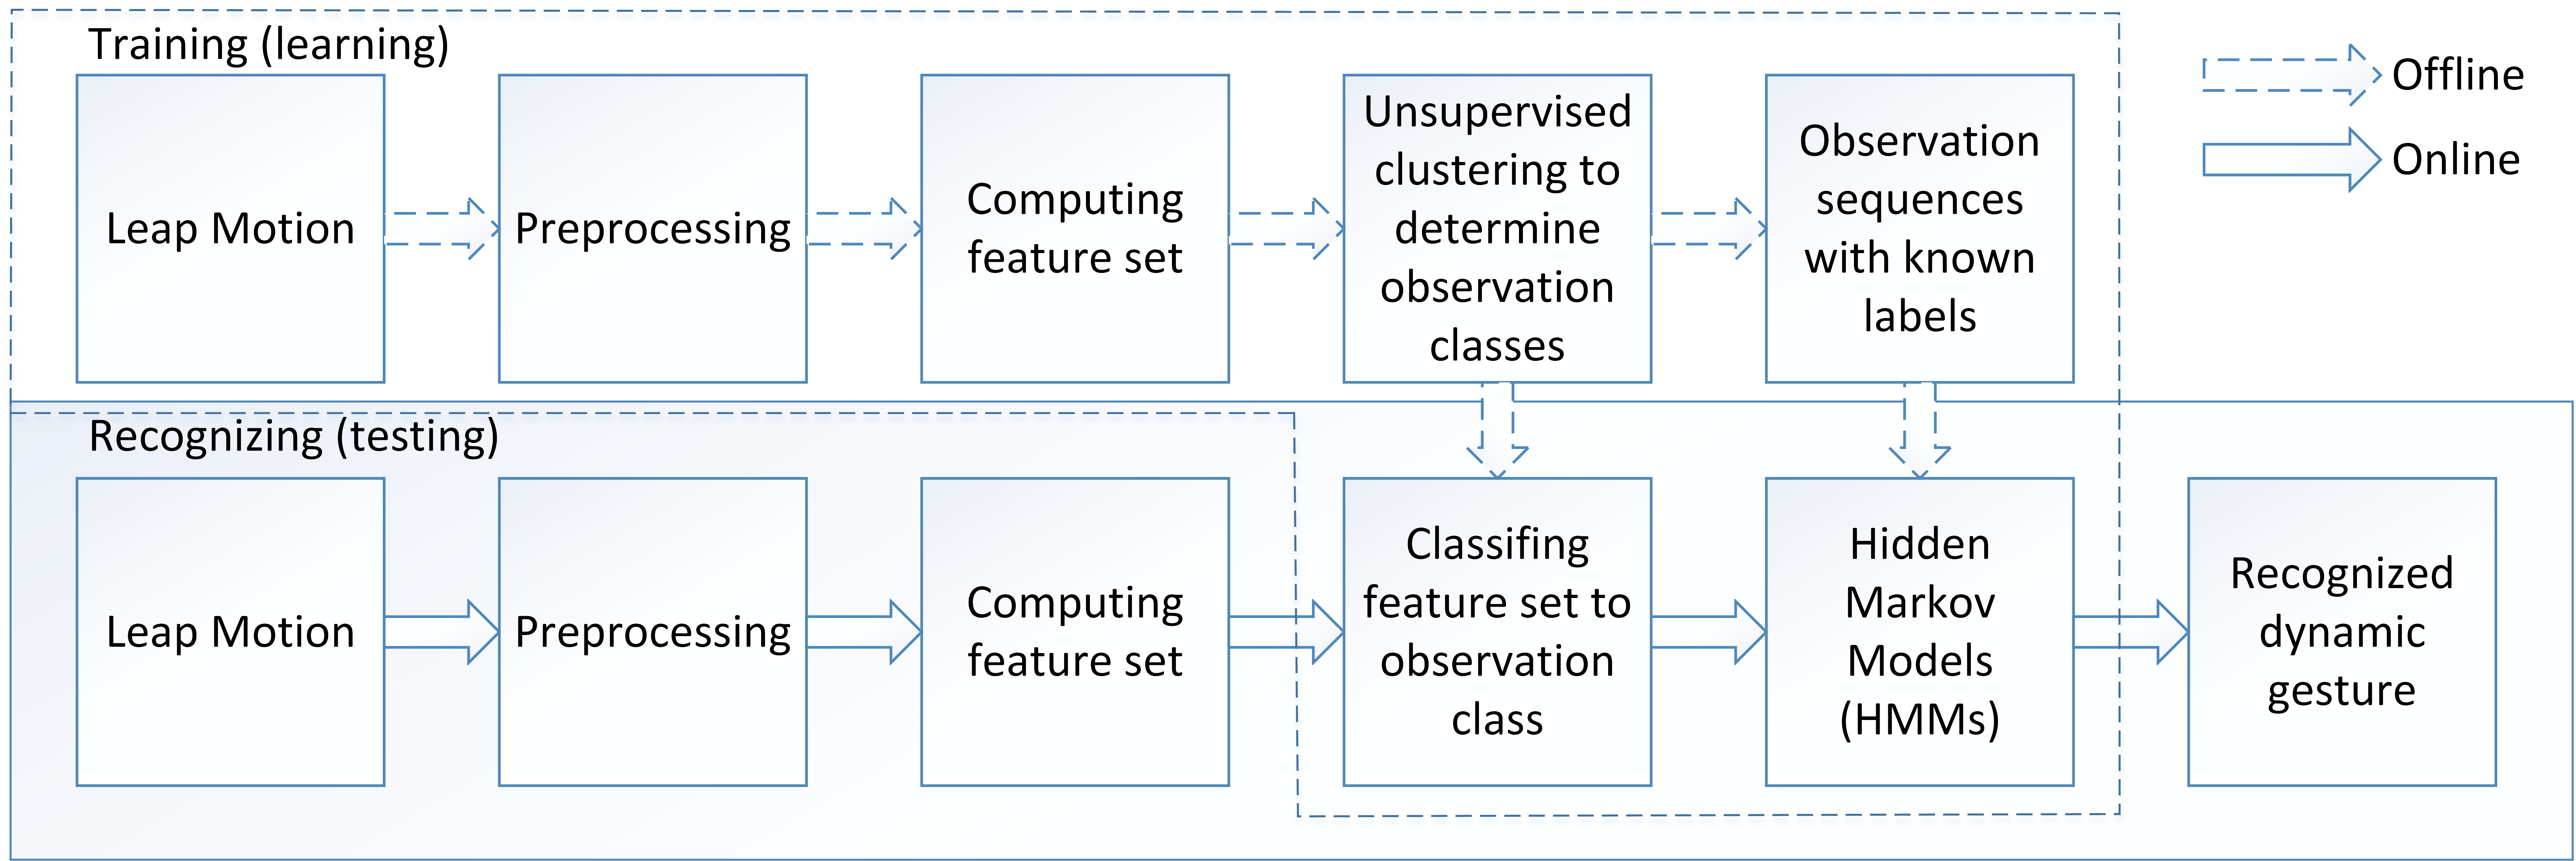
\includegraphics[width=1\columnwidth]{figures/DynamicGestures.png}
 \caption{Solution blocks of learning and testing parts in task of dynamic gesture recognition}
 \label{dynamicgesturesflow}
\end{figure}

Finally, the whole processing flow has been designed and is presented at fig.~\ref{dynamicgesturesflow}.
The whole solution consists of two parts: off-line learning and on-line recognition.
For learning, the raw data is preprocessed and then the feature are extracted. 
Similarly to the static gestures, the features set were computed. 
In training part, those features are extracted from all recorded positions for all dynamic gestures.
Then one of the unsupervised clustering algorithms is used to find the classes of observations.
Knowledge of the classes is used to represent each dynamic gesture as a series of one-dimensional observations.
After that for each dynamic gesture, the corresponding HMM is learned by running the Baum-Welch algorithm on the sequence of observations.
The Baum-Welch algorithm finds the matrices that maximizes the likelihood for one sequence of observations, therefore the problem of training on multiple training data was encountered.
Following by the idea presented in \cite{hmmtutorial}, each matrix trained by one training example is incorporated into trained matrix by using simple addition with learning rate $\mu$.
Denoting the transition matrix by $T$ and learnt transition matrix $T_{new}$, it can be written:
\begin{equation}\label{eq:dynT}
T = (1-\mu) \times T + \mu \times T_{new}
\end{equation}
The same idea applies also to the emission matrix $E$ and learnt emission matrix $E_{new}$:
\begin{equation}\label{eq:dynE}
E = (1-\mu) \times E + \mu \times E_{new}
\end{equation}
The problem with the matrices by computing equations\ref{eq:dynT, eq:dynE} is the fact, that they do not represent the probability as the total values do not add to $1.0$.
Therefore, each row of new matrices is normalized to $1.0$.
When dealing with multiple training examples, the resulting solution may be overfitted to the training samples.
To deal with this problem, the K-fold cross validation was utilized in a similar approach as in the static gestures.
To complete the training process, each of the HMMs is put into one recognition structure. 
During the recognition part, observed sequence is treated as input to the Viterbi algorithm performed on each of the HMMs and the output is analysed.
The HMM with the highest likelihood is chosen, and the observed sequence is labelled with the label of this HMM.

In the on-line working, the raw data from leap motion is preprocessed, then each frame is labelled accordingly to the classes learnt by the unsupervised clustering algorithm.
The next step include providing the set of observations to HMM and running the Viterbi algorithm.
The Viterbi algorithm finds the most likely sequence in one the parallel paths, which informs us about the number of the found gesture. 
If the likelihood is above threshold, the gesture is assumed to be correctly recognized.


\section{Evaluation methodology}

To evaluate the quality of recognition achieved by proposed processing pipeline, $6$ dynamic gesture were chosen for which the data was recorded.
For each of those gestures, we recorded 120 samples (30 samples per each author).
The recorded data were also recorded in different positions with respect to the Leap Motion coordinate system and with different speed to measure the wanted invariance and robustness.
The chosen dynamic gestures are:
\begin{enumerate}
\item ``123'' -- it's a gesture when performing counting to 3 using hands,
\item ``door'' -- it's a gesture performed while trying to grasp a handle of door and then open the door,
\item ``circle'' -- making a circle in the air with the forefinger,
\item ``scissors'' -- simulating the cutting with the scissors made by a forefinger and a middle finger,
\item ``gun'' -- only the thumb and the index finger are not in the fist. The hand moves up simulating the movement during the firing from the gun.
\item ``moving the object'' -- performing the task of grasping an invisible object, moving it and letting it go in different place.
\end{enumerate}

To test the proposed approach, similarly to the static gesture recognition problem, the $120\times6=720$ samples were divided into training set containing $66,7\%$ of recordings and testing group containing the remaining $240$ recordings. 
The part of the gestures recorded by Katarzyna were used to find the proper number of clusters than could be used by form the observations for the HMMs. 
The training set was used to train each HMM separately on the training data of each gesture.
Preliminary results revealed that initialization of HMM matrices has an impact on the achieved results.
Due to no prior knowledge, the random initialization was chosen.
This approach did not yield reliable solutions in all situation and therefore each training process is performed $10$ times and the best model from cross-validation is returned.  
Each training cycle of all HMMs takes between $1-10$ minutes, with total training part taking around $25-45$ minutes.
If not stated otherwise, the learning rate $\mu$ was set to $0.1$, k-cross validation was performed for $k=5$ and the number of states in one HMM was set to $10$.


\section{Experiments}


The performed experiments started with testing the unsupervised clustering methods to determine the correct number of observations.
Based on the successful static gesture recognition, each of the hand poses was represented by the vector of values containing:
\begin{itemize}
\item number of detected fingers,
\item $5$ greatest angles between the finger tip vector and palm normal,
\item $5$ greatest angles between the fingers tip vectors,
\item $5$ greatest distances between the tip positions of fingers.
\end{itemize}
In order to compare different hand poses, the distance function was introduced as the L2 norm between feature vectors:
\begin{equation}
d(x,y) = \sqrt{ \sum_{i=1}^{16} (x_i - y_i)^2 }
\end{equation}
The Chinese whispers and Girven-Newman uses the similarity function, which was defined as: 
\begin{equation}
s(x,y) = \frac{1.0}{ \max{\{d(x,y), eps\}}}
\end{equation}
where $eps$ was the numerical epsilon.

For the Chinese Whispers and Girven-Newman clustering the typical parameters from dlib-ml library were used --- the Chinese Whispers maximal iterations were set to $100$, while the Girven-Newman was run with maximal iterations equal to $2000$ and precision eps was set to $1e-4$.
For the SSE analysis for different cluster number, the publicly available script was used\cite{SSE}. 
The script automatically calculates the k-means clustering algorithm for chosen range of $k$ values and presents the figures, which can be a help in determining the correct number of classes.
For the Silhouette width analysis own, R script was written.



\begin{figure}[htp!]
\centering
 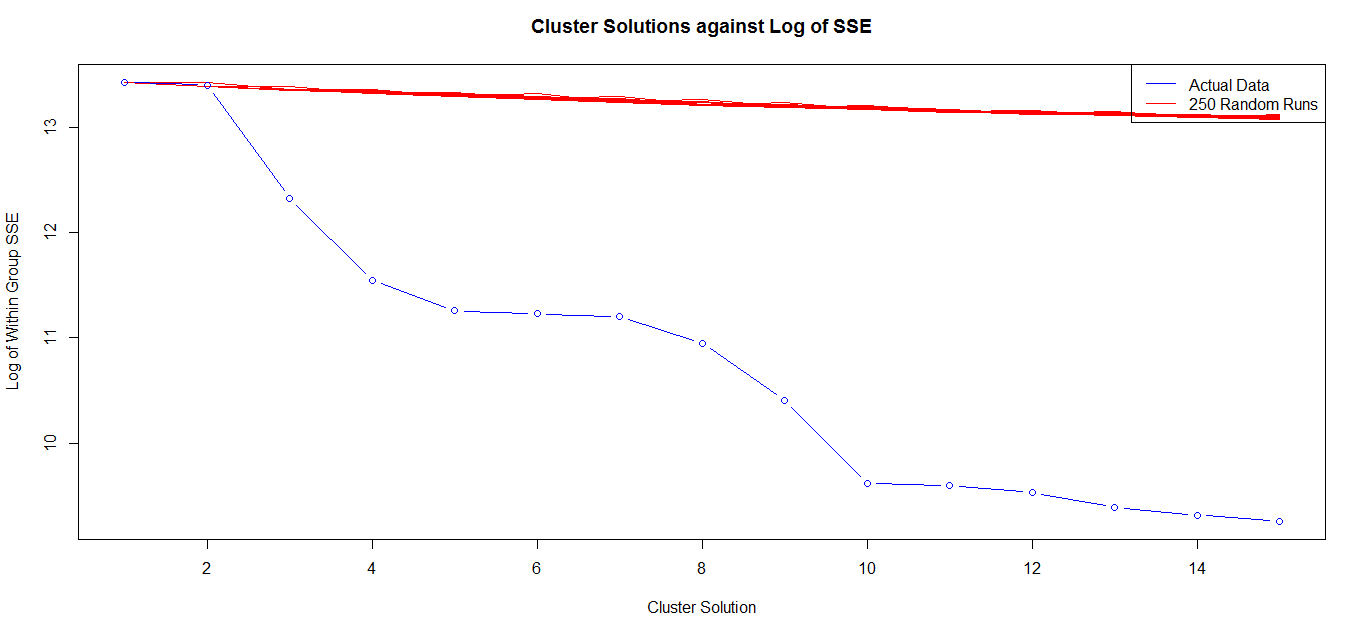
\includegraphics[width=1.0\columnwidth]{figures/SSE1.png}
 %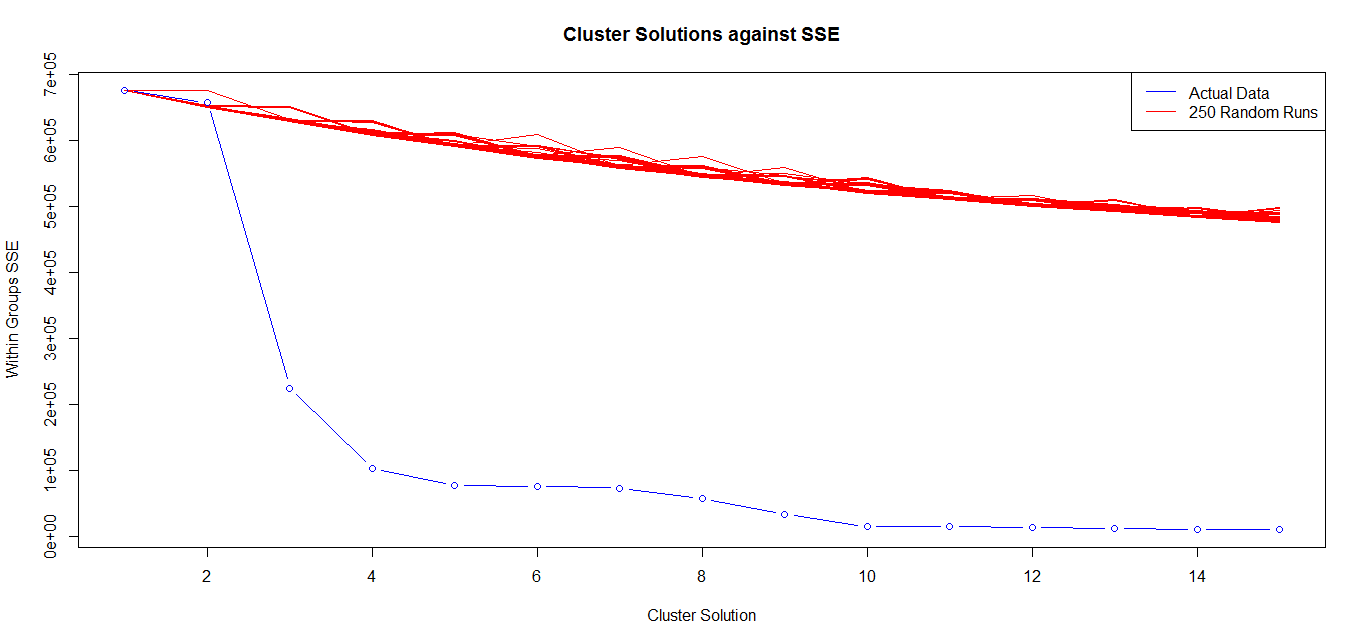
\includegraphics[width=0.7\columnwidth]{figures/SSE2.png}
 %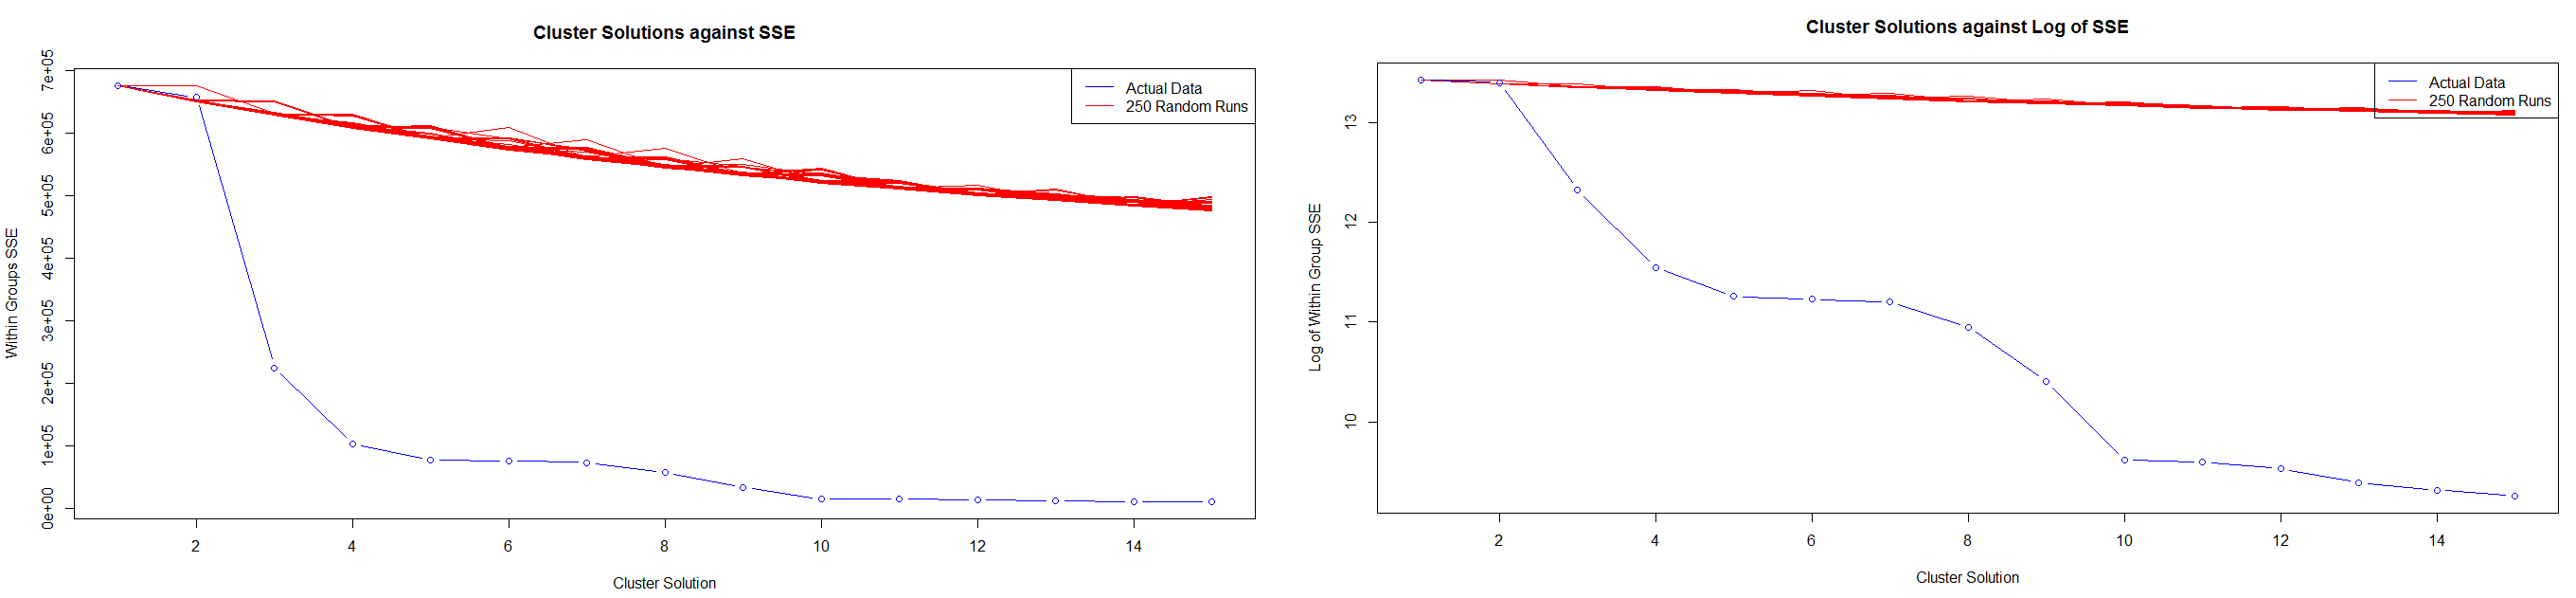
\includegraphics[width=1\columnwidth]{figures/SSE.png}
 \caption{Different representations of SSE as a function of number of clusters for the k-means algorithm}
 \label{dynamicSSE}
\end{figure}

The SSE analysis usually does not yield the direct answer.
The tool provides several plots, but the most interesting one is presented at fig.~\ref{dynamicSSE}. 
Looking at this plot, there is a significant drop in SSE for the cluster number equal to $5$ and $10$.
It is expected that either of those numbers is the correct choice when it comes to the number of classes for k-means algorithm.
The Silhouette width approach estimated that the there are $4$ distinguishable classes in recorded gestures.


\begin{table}[ht]
 \caption{Comparison of suggested number of clusters for the dataset containing all positions of hand in all dynamic gesture recordings made by Katarzyna}
 \label{clusterwyn}
    \begin{tabular}{ccccc}
    \hline
     & Girven-Newman & Chinese whispers   & SSE vs clusters & Silhouette width  \\ \hline
    recordings \\by Katarzyna          & -      & $613$ & $5$ or $10$     & $4$     \\ \hline
    \end{tabular}
\end{table}

The proposed values of clusters for different methods are presented in the table~\ref{clusterwyn}.
The Girvan-Newman algorithm did not provide any estimate within $24$ hours and therefore was considered impractical.
Due to the inconclusive results, the correct number of classes was decided to be determined by performing experiments with different class number parameter.
The analysis of the correct class number was postponed until the correct feature set is chosen.
Until stated otherwise, the class number equal to $10$ was chosen.

The next challenge was to find the feature set describing one gesture in time, that would contain the information about the dynamic nature of the gesture to be recognized. 
The first feature set consisted of features encoding the information about the speed of the hand. For each $i-th$ hand position in recorded sequence, the $(i-10)$-th position was also considered. 
The feature set consisted of the recorded displacement of hand in $X$, $Y$, $Z$ directions.
The number of fingers in both positions were also added, resulting in feature set containing:
\begin{itemize}
\item finger count in $i$-th hand position,
\item finger count in $i-10$-th hand position,
\item displacement of hand position in $X$,
\item displacement of hand position in $Y$,
\item displacement of hand position in $Z$.
\end{itemize}
The presented approach allowed to achieve $64.583\%$ on cross-validation set. 
Due to the small testing set, the total recognition rate was calculated on training and testing sets.
This approach resulted in $61.806\%$ on all samples, which is too small to by used in real applications.

The previous approach suffered from the fact, that the encoded speeds are represented in the coordinate system of the Leap Motion.
Executing the gesture with different angle to the Leap Motion's coordinate system makes the recognition tasks harder and sometimes results in mislabelling.
Therefore, the feature set was supposed to encode the information with respect to the local coordinate system of hand. 
In new approach, the magnitude of the displacement is calculated. 
It is independent of the chosen orientation of the coordinate system.
To represent the direction of movement, the normalized displacement vector is computed as a vector connecting the center of $i-10$-th hand position with $i$-th hand position.
Then, the dot product between normalized displacement vector and palm normal in $i-10$ position is calculated.
As this not encode the whole information, the dot product between the normalized displacement vector and the plan direction is also computed.
The resulting feature contains also $5$ elements:
\begin{itemize}
\item finger count in $i$-th hand position,
\item finger count in $i-10$-th hand position,
\item magnitude of the hand's displacement,
\item dot product of the normalized displacement vector and the palm's normal in $i-10$-th position,
\item dot product of the normalized displacement vector and the palm's direction in $i-10$-th position.
\end{itemize}
This approach allowed to improve the recognition rate in cross-validation ($69.583\%$) and on the whole set ($67.500\%$), although was still not satisfying from the practical point of view.

The simple observation on the feature set and recorded gestures reveals that sometimes only the fingers are changing positions, while position of hand is steady.
The previous approaches, did not encode this information in feature vectors, which made the those changes invisible to the further processing pipeline.
Therefore, the new feature vector contained also the information about the displacement of each corresponding finger.
In order to keep the feature size small, it was decided to only incorporate the magnitude of those displacements. 
Due to the nature of Leap Motion's erratic numbering of fingers, those magnitudes were also sorted.
The total of 4 top values were added to feature vector resulting in:
\begin{itemize}
\item finger count in $i$-th hand position,
\item finger count in $i-10$-th hand position,
\item magnitude of the hand's displacement,
\item dot product of the normalized displacement vector and the palm's normal in $i-10$-th position,
\item dot product of the normalized displacement vector and the palm's direction in $i-10$-th position,
\item $4$ greatest magnitudes of finger displacements.
\end{itemize}
The results were not satisfying as were even worse than the ones achieved for the feature set 2 -- $66.111\%$ compared to the previously received $67.500\%$. 
The further inspection revealed that, while adding displacement of fingers helps in most situations, it can also pose a great risk.
In case of different order of finger numbering, the resulting displacement may be calculated between different fingers, thus resulting in big artificial displacement of fingers.
Therefore, the idea of using displacement of fingers was abandoned.
 
Looking at the recorded gestures, it seemed that speed information is not sufficient to correctly detect the sequences of gestures combining in one dynamic gesture.
The new feature set, contained also the information about the static hand positions allowing to distinguish dynamic gestures that are comprised of sequential static gestures.
The new feature set contained the already proposed speed part with additional static encoding that was successfully used in static gesture recognition:
\begin{itemize}
\item finger count in $i$-th hand position,
\item finger count in $i-10$-th hand position,
\item magnitude of the hand's displacement,
\item dot product of the normalized displacement vector and the palm's normal in $i-10$-th position,
\item dot product of the normalized displacement vector and the palm's direction in $i-10$-th position,
\item $4$ greatest euclidean distances between all combination of finger's tips in $i$-th position,
\item $4$ greatest absolute angles between all combination of finger's vectors in $i$-th position,
\item $4$ greatest euclidean distances between finger's tips and palm's position in $i$-th position,
\item $4$ greatest absolute angles between finger's vectors and palm's normal in $i$-th position.
\end{itemize}

The experiments showed that the proposed approach is not as successful as it was believed.
It was believed that the sophisticated static part of feature set is dominating dynamic part of feature set, which prevents the method from achieving better results.
Therefore, the $5$-th proposed feature set consist of static part represented by the $4$ greatest euclidean distances between all combination of finger's tips in $i$-th position and $4$ greatest absolute angles between all combination of finger's vectors in $i$-th position.
Similarly, feature sets $6$, $7$, $8$ were also the propositions containing the reduced static parts, but did not improve significantly over already received results. 
The results obtained by all proposed feature sets are presented in tab.~\ref{tab:dyn1}. 

\begin{table}[htp!]
	\label{tab:dyn1}
	\caption{Results obtained by the HMM approach using different feature sets, 10 classes}
    \begin{tabular}{|c|c|c|}
    \hline
    ~                                 & 5 gestures, CV & 5 gestures, whole dataset  \\ \hline
    feature set 1                     & 64.583\% & 61.806\%   \\ \hline
    feature set 2                     & 69.583\% & 67.500\%   \\ \hline
    feature set 3                     & 68.542\% & 66.111\%   \\ \hline
    feature set 4,          		  & 77.917\% & 76.111\%   \\ \hline
    feature set 5                     & 66.667\% & 63.889\%   \\ \hline
    feature set 6,                    & 72.912\% & 70.417\%   \\ \hline
    feature set 7,                    & 71.875\% & 69.167\%   \\ \hline
    feature set 8,                    & 78.125\% & 77.222\%   \\ \hline
    \end{tabular}
\end{table}
  
The best results were obtained for feature set $8$, but the results obtained by the full static representation (feature set $4$) are not significantly worse.
For further assessment, the feature set $4$ was chosen as the one that describes each gesture with more information and therefore is believed to work better for gestures that were not included in proposed experiments.

The next experiments were performed to test what is the best number of observation classes for k-means algorithm. 
The tests were conducted using feature set $4$ and learning rate $\mu=0.05$.

\begin{table}[htp!]
	\label{tab:dyn1}
	\caption{Results obtained by the HMM approach using feature set 4 and different class clusters}
    \begin{tabular}{|c|c|c|}
    \hline
    ~                                 & 5 gestures, CV & 5 gestures, whole dataset  \\ \hline
	k = 4                  	  & 77.292\% & 74.722\%   \\ \hline
    k = 5               	  & 79.583\% & 77.639\%   \\ \hline
    k = 6                     & 79.583\% & 77.639\%   \\ \hline
    k = 8                     & 77.708\% & 75.977\%   \\ \hline
    k = 10                    & 77.917\% & 76.111\%   \\ \hline
    k = 12                    & 78.542\% & 77.361\%   \\ \hline
    \end{tabular}
\end{table}
The best obtained results are for the $k=5$ and $k=6$ allowing to increase of the recognition rate from cross-validation to $79.583\%$ and increase to the $77.639\%$ on the whole dataset. 

The next experiments involved finding the best learning rate. 
In our application, the stable learning rate was chosen to minimize the number of parameters to tune. 
The further developments may involve using learning rate that is changing depending on the already received learning rate.
Using predefined learning rate may be dangerous as small value may mean small convergence, while too big step may result in not converging to the locally best solution. 
The achieved results are presented in~\ref{tab:dyn2}.
In proposed application, the learning rate $\mu = 0.05$ allowed to achieve the best results. 

\begin{table}[htp!]
	\label{tab:dyn2}
	\caption{Results obtained by the HMM approach using feature set 4, 5 observation classes and different learning rates}
    \begin{tabular}{|c|c|c|}
    \hline
    ~                                 & 5 gestures, CV & 5 gestures, whole dataset  \\ \hline
	$\mu$ = 0.01                  	  & 77.500\% & 76.944\%   \\ \hline
    $\mu$ = 0.05                      & 80.417\% & 79.028\%   \\ \hline
    $\mu$ = 0.1                      & 79.583\% & 77.639\%   \\ \hline
    $\mu$ = 0.2                      & 69.583\% & 69.7222\%   \\ \hline
    \end{tabular}
\end{table}


The only parameter not tested in previous experiments is the number of state each HMM is composed of. 
The previously used value was equal to $10$ states.
The performed experiments confirmed the choice as smaller number of states ($5$) resulted in lower recognition rate, while greater number of states did not improve the result.
The drawback of taking HMMs with big state numbers is the learning time. 
The performed experiments and theoretical computational complexity confirm that the computational complexity grows linear with the chosen number of states, which in practical applications means linear grow of taken processing time.


\begin{table}[htp!]
	\label{tab:dyn3}
	\caption{Results obtained by the HMM approach using feature set 4, 6 observation classes and different state elements}
    \begin{tabular}{|c|c|c|}
    \hline
    ~                                 & 5 gestures, CV & 5 gestures, whole dataset  \\ \hline
	K = 5                  	  & 73.958\% & 73.611\%   \\ \hline
    K = 10                     & 79.583\% & 77.639\%   \\ \hline
    K = 20                    & 77.500\% & 76.528\%   \\ \hline
    K = 30                     & 77.917\% & 76.25\%   \\ \hline
    \end{tabular}
\end{table}

